%================================================
% TASK 2.1
%================================================
\section{Task 2.1: Percentage of Cancelled Orders per City}

\subsection{Phân tích truy vấn}

Bài toán yêu cầu tính \textbf{phần trăm đơn hàng bị hủy} theo từng thành phố (\texttt{ship-city}), trong đó chỉ xét các đơn hàng thỏa mãn \textbf{đồng thời ba điều kiện} sau:

\textbf{Điều kiện 1 --- Mức dịch vụ.}
Đơn hàng phải có mức dịch vụ giao hàng \texttt{ship-service-level} bằng \texttt{"Standard"}. Trong mã nguồn, phép so sánh được chuẩn hóa bằng \texttt{lower(trim(col("ship-service-level"))) === "standard"} để tránh sai lệch do khoảng trắng thừa hoặc khác biệt giữa chữ hoa và chữ thường.

\textbf{Điều kiện 2 --- Có ít nhất 3 khuyến mãi hợp lệ về mặt thời gian.}
Mỗi đơn hàng chứa cột \texttt{promotion-ids}, là chuỗi các mã khuyến mãi được phân tách bằng dấu phẩy. Một chương trình khuyến mãi được gọi là \textit{hợp lệ về mặt thời gian} nếu khoảng thời gian hoạt động của nó trên \textbf{toàn bộ tập dữ liệu} kéo dài ít nhất 2 ngày. Cụ thể, với mỗi mã khuyến mãi duy nhất xuất hiện trong bộ dữ liệu:
\begin{itemize}
    \item Xác định ngày xuất hiện \textbf{đầu tiên} ($d_{\min}$) và ngày xuất hiện \textbf{cuối cùng} ($d_{\max}$).
    \item Tính khoảng thời gian hoạt động: $\text{active\_days} = d_{\max} - d_{\min}$ (tính bằng số ngày).
    \item Khuyến mãi hợp lệ khi và chỉ khi $\text{active\_days} \geq 2$.
\end{itemize}
Một đơn hàng thỏa mãn điều kiện này nếu trong danh sách \texttt{promotion-ids} của nó chứa \textbf{ít nhất 3} mã khuyến mãi hợp lệ, kể cả các khuyến mãi do Amazon phát hành.

\textbf{Điều kiện 3 --- Giá trị đơn hàng (Amount) thấp hơn mức trung bình của bang.}
Tính giá trị trung bình cột \texttt{Amount} theo từng bang \texttt{ship-state} trên tập con các đơn hàng thỏa mãn \texttt{Fulfilment = "Merchant"} và \texttt{Courier Status = "Shipped"}. Đơn hàng đang xét chỉ được giữ lại nếu:
\[
\texttt{Amount}_{\text{order}} < \overline{\texttt{Amount}}_{\text{Merchant,Shipped}}^{\text{(cùng bang)}}
\]

\textbf{Tính phần trăm đơn hàng bị hủy.}
Sau khi lọc ra tất cả đơn hàng thỏa mãn đồng thời cả ba điều kiện trên, chương trình tiến hành gom nhóm theo thành phố \texttt{ship-city} đã được chuẩn hóa để tính toán:
\[
\texttt{cancelled\_percentage} = \frac{|\{o : \texttt{Status}(o) = \text{``Cancelled''}\}|}{|\text{tổng số đơn hàng hợp lệ}|} \times 100
\]
Mã nguồn xác định trạng thái đơn hàng bị hủy bằng phép so khớp \texttt{lower(trim(col("Status"))) === "cancelled"} để đảm bảo tính chính xác sau khi chuẩn hóa.

\textbf{Cấu trúc dữ liệu đầu ra:}
\begin{table}[H]
\centering
\begin{tabular}{lll}
\toprule
\textbf{Cột} & \textbf{Kiểu} & \textbf{Ý nghĩa} \\
\midrule
\texttt{ship-city}  & String & Thành phố giao hàng đã chuẩn hóa viết hoa \\
\texttt{cancelled\_percentage} & Double & Tỷ lệ hủy (\%), làm tròn 4 chữ số thập phân \\
\bottomrule
\end{tabular}
\caption{Định nghĩa schema tệp đầu ra Task\_2-1.parquet}
\label{tab:task2_1_schema}
\end{table}

% ------------------------------------------------------------------
\subsection{Phân rã thành các bước cơ bản}

Lời giải được phân rã thành 9 bước xử lý tuần tự, mỗi bước tương ứng với một phép biến đổi DataFrame rõ ràng:

\begin{enumerate}
    \item \textbf{Đọc dữ liệu CSV và chuyển kiểu dữ liệu} (\texttt{df}).
    Đọc tệp CSV với dòng đầu chứa tiêu đề, tắt tính năng tự động suy luận kiểu dữ liệu (\texttt{inferSchema}) để kiểm soát kiểu dữ liệu một cách chủ động. Phân tích cột \texttt{Date} sang kiểu ngày (\texttt{date}) theo định dạng \texttt{MM-dd-yy}, chuyển kiểu cột \texttt{Amount} sang \texttt{DoubleType}, chuẩn hóa tên thành phố \texttt{ship-city} và bang \texttt{ship-state} bằng hàm \texttt{upper(trim(...))}, đồng thời tạo cột định danh \texttt{order\_row\_id} bằng hàm \texttt{monotonically\_increasing\_id()} để định danh duy nhất cho từng đơn hàng sau các phép liên kết. DataFrame này được lưu tạm vào bộ nhớ (\texttt{cache()}) vì sẽ được tái sử dụng trong nhiều nhánh xử lý khác nhau.

    \item \textbf{Tách các mã khuyến mãi thành từng dòng riêng} (\texttt{promoExploded}).
    Lọc bỏ các dòng có cột \texttt{promotion-ids} rỗng hoặc mang giá trị null. Sử dụng hàm \texttt{split} để tách chuỗi khuyến mãi theo dấu phẩy, dùng hàm \texttt{transform} kết hợp với \texttt{trim} để loại bỏ khoảng trắng dư thừa của từng mã, sau đó dùng hàm \texttt{explode} để phân rã danh sách thành từng dòng mã khuyến mãi riêng lẻ. Bước này rất quan trọng vì khoảng thời gian hoạt động là thuộc tính mang tính chất toàn cục của từng mã khuyến mãi — cần thu thập toàn bộ các ngày xuất hiện của mã trên toàn bộ tập dữ liệu.

    \item \textbf{Tính toán thời gian hợp lệ của khuyến mãi} (\texttt{promoValidity}).
    Gom nhóm theo mã khuyến mãi \texttt{promo\_id}, tính ngày xuất hiện sớm nhất \texttt{min(parsed\_date)} và muộn nhất \texttt{max(parsed\_date)}, sau đó sử dụng hàm hiệu ngày \texttt{datediff} để tính số ngày hoạt động \texttt{active\_days}. Chỉ giữ lại các mã khuyến mãi có số ngày hoạt động $\text{active\_days} \geq 2$.

    \item \textbf{Đếm số khuyến mãi hợp lệ theo từng đơn hàng bằng DataFrame}.
    Từ DataFrame gốc \texttt{df}, chương trình thực hiện phân rã các mã khuyến mãi theo định danh đơn hàng \texttt{order\_row\_id}, liên kết với bảng khuyến mãi hợp lệ \texttt{promoValidity}, sau đó gom nhóm theo \texttt{order\_row\_id} để đếm số lượng khuyến mãi hợp lệ duy nhất bằng hàm \texttt{countDistinct}. Cách làm này giữ nguyên tính chất declarative của Structured API, không sử dụng hàm tự định nghĩa (UDF) và không phải thu thập dữ liệu về nút điều phối, giúp Catalyst dễ dàng tối ưu hóa.

    \item \textbf{Áp dụng Điều kiện 1 và 2} (\texttt{afterCond12}).
    Lọc các đơn hàng có \texttt{ship-service-level = "Standard"}, sau đó thực hiện phép liên kết trái với bảng đếm số khuyến mãi hợp lệ \texttt{validPromotionCounts} theo \texttt{order\_row\_id}; các đơn hàng không có khuyến mãi nào hợp lệ sẽ nhận giá trị mặc định là \texttt{0} thông qua hàm \texttt{coalesce}. Cuối cùng, thực hiện lọc lấy các đơn hàng có \texttt{valid\_promo\_count >= 3}.

    \item \textbf{Tính toán giá trị trung bình Amount theo bang} (\texttt{stateAvgDf}).
    Từ DataFrame gốc \texttt{df} (không phải \texttt{afterCond12}), lọc các bản ghi có \texttt{Fulfilment = "Merchant"} và \texttt{Courier Status = "Shipped"}, loại bỏ các dòng có giá trị Amount bị null, sau đó thực hiện gom nhóm và tính trung bình: \texttt{groupBy("ship\_state\_norm").agg(avg("Amount"))}. Kết quả thu được là một bảng dữ liệu nhỏ chứa ngưỡng chi tiêu trung bình cho từng bang.

    \item \textbf{Liên kết và áp dụng Điều kiện 3} (\texttt{qualifiedDf}).
    Thực hiện phép liên kết trong giữa \texttt{afterCond12} và \texttt{stateAvgDf} trên cột bang \texttt{ship\_state\_norm}, sau đó lọc lấy các đơn hàng có \texttt{Amount < merchant\_shipped\_avg}. Sau bước này, ta thu được tập hợp các đơn hàng thỏa mãn đồng thời cả ba điều kiện lọc.

    \item \textbf{Tính phần trăm đơn hàng bị hủy theo từng thành phố} (\texttt{resultDf}).
    Gom nhóm theo thành phố \texttt{ship\_city\_norm}, đếm tổng số đơn hàng bằng \texttt{count(*)} và đếm số đơn hàng bị hủy bằng hàm tổng điều kiện \texttt{sum(when(... === "cancelled", 1).otherwise(0))}. Tính tỷ lệ phần trăm đơn hàng bị hủy và làm tròn đến 4 chữ số thập phân.

    \item \textbf{Xuất tệp Parquet duy nhất}.
    Sử dụng \texttt{coalesce(1)} để gom dữ liệu về một phân vùng duy nhất, ghi vào một thư mục tạm trên ổ đĩa, sau đó đổi tên tệp bộ phận thành tên tệp Parquet đơn lẻ chính xác theo đường dẫn đầu ra và dọn dẹp các tệp phụ checksum.
\end{enumerate}

% ------------------------------------------------------------------
\subsection{Lý do phân rã}

\textbf{Tính khoảng hoạt động hợp lệ của khuyến mãi trên toàn bộ tập dữ liệu trước.}
Khoảng thời gian hoạt động của một mã khuyến mãi được xác định bởi khoảng cách giữa ngày xuất hiện đầu tiên và ngày xuất hiện cuối cùng của nó trên toàn bộ tập dữ liệu, chứ không thể chỉ xét riêng lẻ trong từng đơn hàng. Do đó, quy trình phân rã-gom nhóm-hiệu ngày bắt buộc phải được xử lý trên toàn bộ dữ liệu trước khi áp dụng ngược lại cho từng đơn hàng. Đây là lý do quy trình xử lý được chia thành hai nhánh song song: một nhánh tính toán độ hợp lệ của các mã khuyến mãi và nhánh chính xử lý dữ liệu đơn hàng.

\textbf{Ngưỡng chi tiêu trung bình theo bang phải được tính riêng rồi liên kết sau.}
Điều kiện thứ ba yêu cầu so sánh giá trị \texttt{Amount} của mỗi đơn hàng với mức trung bình của bang tương ứng nhưng chỉ trên tập hợp con các đơn hàng của Merchant và đã Shipped. Vì tập hợp con này có tính chất khác biệt hoàn toàn với tập hợp đơn hàng Standard đang xét, chúng ta không thể sử dụng trực tiếp hàm cửa sổ mà bắt buộc phải tính toán trung bình riêng biệt thành bảng \texttt{stateAvgDf} rồi thực hiện phép liên kết theo cột \texttt{ship\_state\_norm}. Vì bảng \texttt{stateAvgDf} có kích thước rất nhỏ, Spark có thể tự động áp dụng phép liên kết phát tán \texttt{BroadcastHashJoin} để tránh chi phí phân tán dữ liệu qua mạng.

\textbf{Thứ tự áp dụng các điều kiện lọc giúp tối ưu hóa chi phí shuffle.}
Mã nguồn chủ động áp dụng Điều kiện 1 (lọc các đơn Standard) trước khi liên kết với bảng đếm số khuyến mãi để giảm thiểu số lượng đơn hàng tham gia vào phép liên kết. Điều kiện 3 (so sánh giá trị trung bình của bang) được áp dụng sau cùng vì nó phụ thuộc vào kết quả liên kết với bảng \texttt{stateAvgDf}. Nếu đảo ngược thứ tự — liên kết với bảng trung bình của bang trước rồi mới lọc mức dịch vụ và khuyến mãi — khối lượng dữ liệu tham gia vào phép liên kết và chi phí shuffle trung gian sẽ tăng lên rất nhiều.

% ------------------------------------------------------------------
\subsection{Chiến lược thực thi \& Triển khai mã nguồn}

Task 2.1 được cài đặt trong file \texttt{src/Task\_2-1/source/Task2\_1.scala}, sử dụng hoàn toàn DataFrame/Dataset API --- tuyệt đối không dùng các chuỗi truy vấn Spark SQL dạng thô. Chương trình nhận hai tham số: đường dẫn CSV đầu vào và đường dẫn file Parquet đầu ra.

\textbf{Lệnh chạy mẫu:}
\begin{lstlisting}[language=bash]
cat > /tmp/task2_1.runner.scala <<'EOF'
:load src/Task_2-1/source/Task2_1.scala
Task2_1.main(Array("data/input/Amazon Sale Report.csv",
  "data/output/Task_2-1.parquet"))
sys.exit(0)
EOF
spark-shell < /tmp/task2_1.runner.scala
\end{lstlisting}

\textbf{Explode và tính promotion validity.}
\begin{lstlisting}[language=Scala]
val promoExploded = df
  .filter(col("promotion-ids").isNotNull
       && col("promotion-ids") =!= "")
  .select(col("parsed_date"),
    explode(transform(
      split(col("promotion-ids"), ","),
      (promoId: Column) => trim(promoId)
    )).as("promo_id"))
  .filter(col("promo_id") =!= "")

val promoValidity = promoExploded
  .groupBy("promo_id")
  .agg(min("parsed_date").as("first_date"),
       max("parsed_date").as("last_date"))
  .withColumn("active_days",
    datediff(col("last_date"), col("first_date")))
  .filter(col("active_days") >= 2)
  .select("promo_id")
\end{lstlisting}

Lý do chương trình sử dụng hàm biến đổi \texttt{transform} kết hợp với \texttt{trim} trước khi chạy \texttt{explode} thay vì cắt khoảng trắng sau khi phân rã là: đảm bảo mỗi mã khuyến mãi được làm sạch ngay trong mảng trước khi phân rã dòng mới, tránh sinh ra các dòng trống vô nghĩa do các dấu phẩy dư thừa ở cuối chuỗi.

\textbf{Đếm valid promotions theo order bằng DataFrame.}
\begin{lstlisting}[language=Scala]
val orderPromos = df
  .filter(col("promotion-ids").isNotNull &&
          trim(col("promotion-ids")) =!= "")
  .select(col("order_row_id"),
    explode(transform(split(col("promotion-ids"), ","),
      (promoId: Column) => trim(promoId))).as("promo_id"))
  .filter(col("promo_id") =!= "")

val validPromotionCounts = orderPromos
  .join(broadcast(promoValidity), Seq("promo_id"), "inner")
  .groupBy("order_row_id")
  .agg(countDistinct("promo_id").as("valid_promo_count"))
\end{lstlisting}

Chiến lược này giữ trọn vẹn tính chất declarative của Structured API. Bảng \texttt{promoValidity} chỉ chứa 185 khuyến mãi hợp lệ nên được Spark tự động phát tán làm nhánh dựng bảng \textbf{Build side} khi liên kết với \texttt{orderPromos}; phần đếm số lượng theo khóa \texttt{order\_row\_id} là phép gom nhóm rõ ràng, hiển thị trực quan trong kế hoạch vật lý.

\textbf{Filter service level và đếm promotions.}
\begin{lstlisting}[language=Scala]
val afterCond12 = df
  .filter(lower(trim(
    col("ship-service-level"))) === "standard")
  .join(validPromotionCounts, Seq("order_row_id"), "left")
  .withColumn("valid_promo_count",
    coalesce(col("valid_promo_count"), lit(0L)))
  .filter(col("valid_promo_count") >= 3)
\end{lstlisting}

\textbf{Tính trung bình Amount theo state.}
\begin{lstlisting}[language=Scala]
val stateAvgDf = df
  .filter(
    lower(trim(col("Fulfilment"))) === "merchant" &&
    lower(trim(col("Courier Status"))) === "shipped")
  .filter(col("Amount").isNotNull)
  .groupBy("ship_state_norm")
  .agg(avg("Amount").as("merchant_shipped_avg"))
\end{lstlisting}

\textbf{Join điều kiện 3 và tính cancelled percentage.}
\begin{lstlisting}[language=Scala]
val joinedDf = afterCond12.join(
  stateAvgDf, Seq("ship_state_norm"), "inner")

val qualifiedDf = joinedDf
  .filter(col("Amount").isNotNull)
  .filter(col("Amount") < col("merchant_shipped_avg"))

val resultDf = qualifiedDf
  .groupBy(col("ship_city_norm"))
  .agg(
    count("*").as("total_orders"),
    sum(when(lower(trim(col("Status"))) === "cancelled",
             1).otherwise(0)).as("cancelled_orders"))
  .withColumn("cancelled_percentage",
    round(col("cancelled_orders") /
          col("total_orders") * 100.0, 4))
  .select(col("ship_city_norm").as("ship-city"),
          col("cancelled_percentage"))
  .orderBy("ship-city")
\end{lstlisting}

Việc chuẩn hóa tên thành phố \texttt{ship-city} trước khi gom nhóm là cực kỳ cần thiết để loại bỏ các sai lệch do chữ hoa/thường và khoảng trắng thừa. Kết quả cuối cùng bám sát yêu cầu của đề bài: tính tỷ lệ phần trăm cho từng thành phố.

% ------------------------------------------------------------------
\subsection{Phân tích chuyên sâu --- Kế hoạch thực thi}

\subsubsection{Đầu ra của lệnh explain(true)}
Dưới đây là kế hoạch thực thi chi tiết thu được từ lệnh \texttt{resultDf.explain(true)} khi chạy chương trình:

\begin{lstlisting}[language={},basicstyle=\ttfamily\tiny]
== Physical Plan ==
AdaptiveSparkPlan isFinalPlan=false
+- Sort [ship-city ASC NULLS FIRST], true, 0
   +- Exchange rangepartitioning(ship-city ASC NULLS FIRST, 200)
      +- HashAggregate(keys=[ship_city_norm], functions=[sum(...), count(1)])
         +- Exchange hashpartitioning(ship_city_norm, 200)
            +- HashAggregate(keys=[ship_city_norm], functions=[partial_sum(...), partial_count(1)])
               +- Project [Status, ship_city_norm]
                  +- BroadcastHashJoin [ship_state_norm], [ship_state_norm], Inner, BuildRight,
                     (Amount < merchant_shipped_avg), false
                     :- Project [Status, Amount, ship_city_norm, ship_state_norm]
                     :  +- BroadcastHashJoin [order_row_id], [order_row_id], Inner, BuildRight, false
                     :     :- Filter lower(trim(ship-service-level)) = standard
                     :     +- BroadcastExchange HashedRelationBroadcastMode(order_row_id)
                     :        +- Filter coalesce(valid_promo_count, 0) >= 3
                     :           +- HashAggregate(keys=[order_row_id],
                     :              functions=[count(distinct promo_id)])
                     :              +- Exchange hashpartitioning(order_row_id, 200)
                     :                 +- HashAggregate(keys=[order_row_id, promo_id])
                     :                    +- Exchange hashpartitioning(order_row_id, promo_id, 200)
                     :                       +- BroadcastHashJoin [promo_id], [promo_id],
                     :                          Inner, BuildRight, false
                     :                          :- Generate explode(transform(split(promotion-ids, ","), trim))
                     :                          +- BroadcastExchange HashedRelationBroadcastMode(promo_id)
                     :                             +- HashAggregate(keys=[promo_id],
                     :                                functions=[min(parsed_date), max(parsed_date)])
                     :                                +- Exchange hashpartitioning(promo_id, 200)
                     +- BroadcastExchange HashedRelationBroadcastMode(ship_state_norm)
                        +- HashAggregate(keys=[ship_state_norm], functions=[avg(Amount)])
                           +- Exchange hashpartitioning(ship_state_norm, 200)
\end{lstlisting}

\subsubsection{Phân tích chiến lược liên kết vật lý}

Quy trình xử lý chứa một phép liên kết chính: \texttt{afterCond12} $\bowtie_{\texttt{ship\_state\_norm}}$ \texttt{stateAvgDf}.

\begin{table}[H]
\centering
\begin{tabular}{p{4cm}lp{6cm}}
\toprule
\textbf{Join} & \textbf{Strategy thực tế} & \textbf{Giải thích} \\
\midrule
\texttt{orderPromos} $\bowtie$ \texttt{promoValidity} & BroadcastHashJoin & \texttt{promoValidity} chỉ có 185 dòng nên được broadcast làm build side. \\
\texttt{standardOrders} $\bowtie$ \texttt{validPromotionCounts} & BroadcastHashJoin & Bảng order đủ điều kiện promotion sau aggregation nhỏ hơn ngưỡng broadcast, Spark chọn BuildRight. \\
\texttt{afterCond12} $\bowtie$ \texttt{stateAvgDf} & BroadcastHashJoin & \texttt{stateAvgDf} chỉ có bảng trung bình theo state, nhỏ hơn nhiều so với broadcast threshold mặc định 10 MB. \\
\bottomrule
\end{tabular}
\caption{Chi tiết các phép liên kết trong kế hoạch thực thi vật lý}
\label{tab:task2_1_joins}
\end{table}

Nhánh dựng bảng \textbf{Build side} của cả ba phép liên kết phát tán \texttt{BroadcastHashJoin} đều nằm ở phía bên phải trong kế hoạch vật lý: \texttt{promoValidity}, \texttt{validPromotionCounts}, và \texttt{stateAvgDf}. Spark tiến hành tuần tự hóa các bảng nhỏ này, phát tán đến các nút thực thi, sau đó thực hiện tìm kiếm bảng băm cục bộ trên phân vùng của bảng lớn hơn. Nhờ đó, các phép liên kết chính không cần phải thực hiện phân tán lại dữ liệu cả hai phía theo khóa liên kết.

Nếu \texttt{stateAvgDf} vượt quá 10 MB (cấu hình mặc định \texttt{spark.sql.autoBroadcastJoinThreshold}), Spark sẽ chuyển sang phép liên kết \texttt{SortMergeJoin} --- yêu cầu shuffle cả hai bảng theo khóa liên kết --- tốn kém hiệu năng hơn rất nhiều. Trong trường hợp cụ thể này, bảng chỉ có $\sim$36 dòng nên BroadcastHashJoin là sự lựa chọn tối ưu nhất.

\subsubsection{Đếm các nút trao đổi dữ liệu}

Dựa trên kế hoạch vật lý thực tế, các nút trao đổi dữ liệu phân tán chính gồm có:

\begin{table}[H]
\centering
\begin{tabular}{clp{6.5cm}}
\toprule
\textbf{\#} & \textbf{Exchange} & \textbf{Mục đích} \\
\midrule
1 & \texttt{hashpartitioning(promo\_id)} & Gom ngày xuất hiện của từng promotion để tính min/max date. \\
2 & \texttt{hashpartitioning(order\_row\_id, promo\_id)} & Khử trùng lặp cặp order--promotion trước khi \texttt{countDistinct}. \\
3 & \texttt{hashpartitioning(order\_row\_id)} & Gom các promotion hợp lệ theo từng order. \\
4 & \texttt{hashpartitioning(ship\_state\_norm)} & Tính trung bình Amount cho Merchant+Shipped theo state. \\
5 & \texttt{hashpartitioning(ship\_city\_norm)} & Gom các đơn qualified theo city để tính percentage. \\
6 & \texttt{rangepartitioning(ship-city)} & Sort toàn cục output cuối. \\
\bottomrule
\end{tabular}
\caption{Phân tích các nút trao đổi dữ liệu và mục đích sử dụng}
\label{tab:task2_1_exchanges}
\end{table}

\textbf{Lưu ý:} Kế hoạch thực thi còn có các nút phát tán \texttt{BroadcastExchange} dành cho các bảng \texttt{promoValidity}, \texttt{validPromotionCounts} và \texttt{stateAvgDf}; đây là cơ chế phát tán bảng nhỏ, hoàn toàn khác với các phép shuffle phân tán dữ liệu của các bảng lớn.

\subsubsection{Đếm các giai đoạn thực thi}

Mỗi nút trao đổi dữ liệu shuffle Exchange sẽ tạo ra một ranh giới phân tách giai đoạn thực thi mới. Với 6 nút shuffle Exchange chính và 3 nút BroadcastExchange, quy trình xử lý kết quả cần khoảng \textbf{7--9 giai đoạn thực thi} cho hành động ghi kết quả đầu ra; số stage thực tế có thể thay đổi nhẹ tùy theo các hành động phụ như \texttt{count()} hay \texttt{show()} phục vụ việc ghi nhật ký.

\begin{enumerate}
    \item \textbf{Stage 1:} Đọc tệp CSV, phân tích ngày tháng và giá trị đơn hàng, duyệt toàn bộ dữ liệu đầu vào.
    \item \textbf{Stage 2:} Phân rã mã khuyến mãi, shuffle theo \texttt{promo\_id}, tính toán ngày bắt đầu và kết thúc.
    \item \textbf{Stage 3:} Lọc đơn hàng Merchant+Shipped, shuffle theo \texttt{ship\_state\_norm}, tính Amount trung bình.
    \item \textbf{Stage 4:} Phân rã khuyến mãi đơn hàng, liên kết phát tán với \texttt{promoValidity}, shuffle theo \texttt{order\_row\_id}.
    \item \textbf{Stage 5:} Lọc mức dịch vụ Standard, thực hiện phép liên kết BroadcastHashJoin với \texttt{validPromotionCounts}.
    \item \textbf{Stage 6:} Thực hiện phép liên kết BroadcastHashJoin với \texttt{stateAvgDf}, lọc giá trị đơn hàng hợp lệ.
    \item \textbf{Stage 7:} Shuffle dữ liệu theo \texttt{ship\_city\_norm}, tính tổng số đơn và đơn bị hủy.
    \item \textbf{Stage 8:} Sắp xếp toàn cục, gộp phân vùng và ghi dữ liệu ra định dạng Parquet.
\end{enumerate}

\subsubsection{Thảo luận về cơ chế tự thích ứng khi thực thi truy vấn}

Trong mã nguồn của Task 2.1, chương trình sử dụng cấu hình mặc định của Spark runtime cho cơ chế tự thích ứng AQE (\texttt{spark.sql.adaptive.enabled}). Với môi trường thực thi Spark 3.4.0, kế hoạch vật lý hiển thị từ khóa \texttt{AdaptiveSparkPlan}, xác nhận AQE đang hoạt động và có thể mang lại các tối ưu hóa sau:
\begin{itemize}
    \item \textbf{Tự động gộp phân vùng sau khi shuffle:} gộp các phân vùng nhỏ sau shuffle, giảm số lượng task dư thừa.
    \item \textbf{Tự động chuyển đổi phép liên kết SortMergeJoin sang BroadcastHashJoin:} nếu sau bước lọc dữ liệu, một bên của phép liên kết có kích thước nhỏ hơn ngưỡng quy định, AQE sẽ tự động chuyển đổi chiến lược liên kết để tối ưu hiệu năng.
    \item \textbf{Tối ưu hóa các phép liên kết bị lệch dữ liệu:} tự động chia nhỏ các phân vùng bị lệch dữ liệu lớn thành nhiều phân vùng nhỏ hơn. Trong quy trình này, phép liên kết trên bang \texttt{ship-state} ít bị ảnh hưởng bởi hiện tượng lệch dữ liệu vì mỗi bang chỉ chứa duy nhất một dòng kết quả trung bình.
\end{itemize}

Trong kế hoạch thực thi minh họa ở trên, dòng chữ \texttt{AdaptiveSparkPlan isFinalPlan=false} xuất hiện do lệnh \texttt{resultDf.explain(true)} được gọi trước khi thực thi hành động ghi dữ liệu đầu ra. Tại thời điểm đó, Spark mới chỉ hiển thị kế hoạch thích ứng ban đầu; AQE vẫn cần thu thập phản hồi trong lúc chạy từ các giai đoạn shuffle trước để đưa ra kế hoạch tối ưu cuối cùng sau khi hành động ghi được thực hiện. Vì vậy, trạng thái \texttt{isFinalPlan=false} hoàn toàn phản ánh đúng nguyên lý hoạt động của AQE.

% ------------------------------------------------------------------
\subsection{Kết quả thực thi \& Xuất dữ liệu}

\begin{itemize}
    \item \textbf{Đường dẫn đầu ra:} \texttt{data/output/Task\_2-1.parquet}.
    \item \textbf{Định dạng:} Tệp Parquet duy nhất, có thể đọc dễ dàng bằng thư viện Pandas (\texttt{pd.read\_parquet}) hoặc Spark ở chế độ chạy cục bộ.
    \item \textbf{Số dòng kết quả:} 2,452 nhóm thành phố.
    \item \textbf{Kích thước tệp:} phụ thuộc vào siêu dữ liệu Parquet của lần ghi dữ liệu thực tế.
\end{itemize}

\textbf{Bảng tổng hợp trích xuất từ tệp Parquet đầu ra:}
\begin{table}[H]
\centering
\begin{tabular}{lr}
\toprule
\textbf{Chỉ số} & \textbf{Giá trị} \\
\midrule
Số dòng kết quả đầu ra & 2,452 \\
Số thành phố duy nhất & 2,452 \\
Giá trị nhỏ nhất của \texttt{cancelled\_percentage} & 0.0 \\
Giá trị lớn nhất của \texttt{cancelled\_percentage} & 0.0 \\
Số thành phố có tỷ lệ đơn bị hủy \texttt{cancelled\_percentage > 0} & 0 \\
\bottomrule
\end{tabular}
\caption{Các chỉ số thống kê tổng quan trích xuất từ tệp Parquet đầu ra của Task 2.1}
\label{tab:task2_1_summary_metrics}
\end{table}

\textbf{Một số dòng kết quả mẫu:}
\begin{lstlisting}[language={}]
ship-city                                      cancelled_percentage
(CHIKMAGALUR DISTERICT).     (N.R PUR THALUKU) 0.0
7BARASAT                                      0.0
ABHAYAPURI                                    0.0
ABOHAR                                        0.0
ABU ROAD                                      0.0
ACHALPUR                                      0.0
ACHANTA                                       0.0
ADAJAN GAM, SURAT                             0.0
ADALAJ                                        0.0
ADBHAR                                        0.0
\end{lstlisting}

\textbf{Kiểm chứng thủ công.}
Chọn thành phố mẫu \texttt{ship-city = BENGALURU}. Sau khi áp dụng đủ ba điều kiện lọc của đề bài, truy vấn kiểm chứng thủ công thu được 1,318 đơn hàng hợp lệ, trong đó không có đơn hàng nào mang trạng thái bị hủy (\texttt{cancelled\_orders = 0}). Các dòng đơn hàng mẫu đều thỏa mãn các mức dịch vụ Standard, số khuyến mãi hợp lệ $\geq 3$ và giá trị đơn hàng nhỏ hơn mức trung bình của bang tương ứng. Do đó:
\[
\texttt{cancelled\_percentage} = \frac{0}{1318} \times 100 = 0.0000
\]
Giá trị này khớp hoàn toàn với kết quả đầu ra \texttt{BENGALURU, 0.0}. Toàn bộ tỷ lệ hủy trong lần chạy dữ liệu hiện tại đều bằng 0 vì không có đơn hàng hợp lệ nào mang trạng thái \texttt{Cancelled}.

% ------------------------------------------------------------------
\subsection{Minh chứng bằng hình ảnh}

Các hình ảnh dưới đây cung cấp minh chứng trực quan về việc chạy chương trình, kế hoạch thực thi Catalyst plan và kết quả kiểm tra tệp dữ liệu đầu ra của Task 2.1.

\begin{figure}[H]
    \centering
    
\includegraphics[width=0.9\textwidth]{img/2-1/run_success.png}
    \caption{Kết quả chạy chương trình Task 2.1}
    \label{fig:task2_1_run_success}
\end{figure}

\begin{figure}[H]
    \centering
    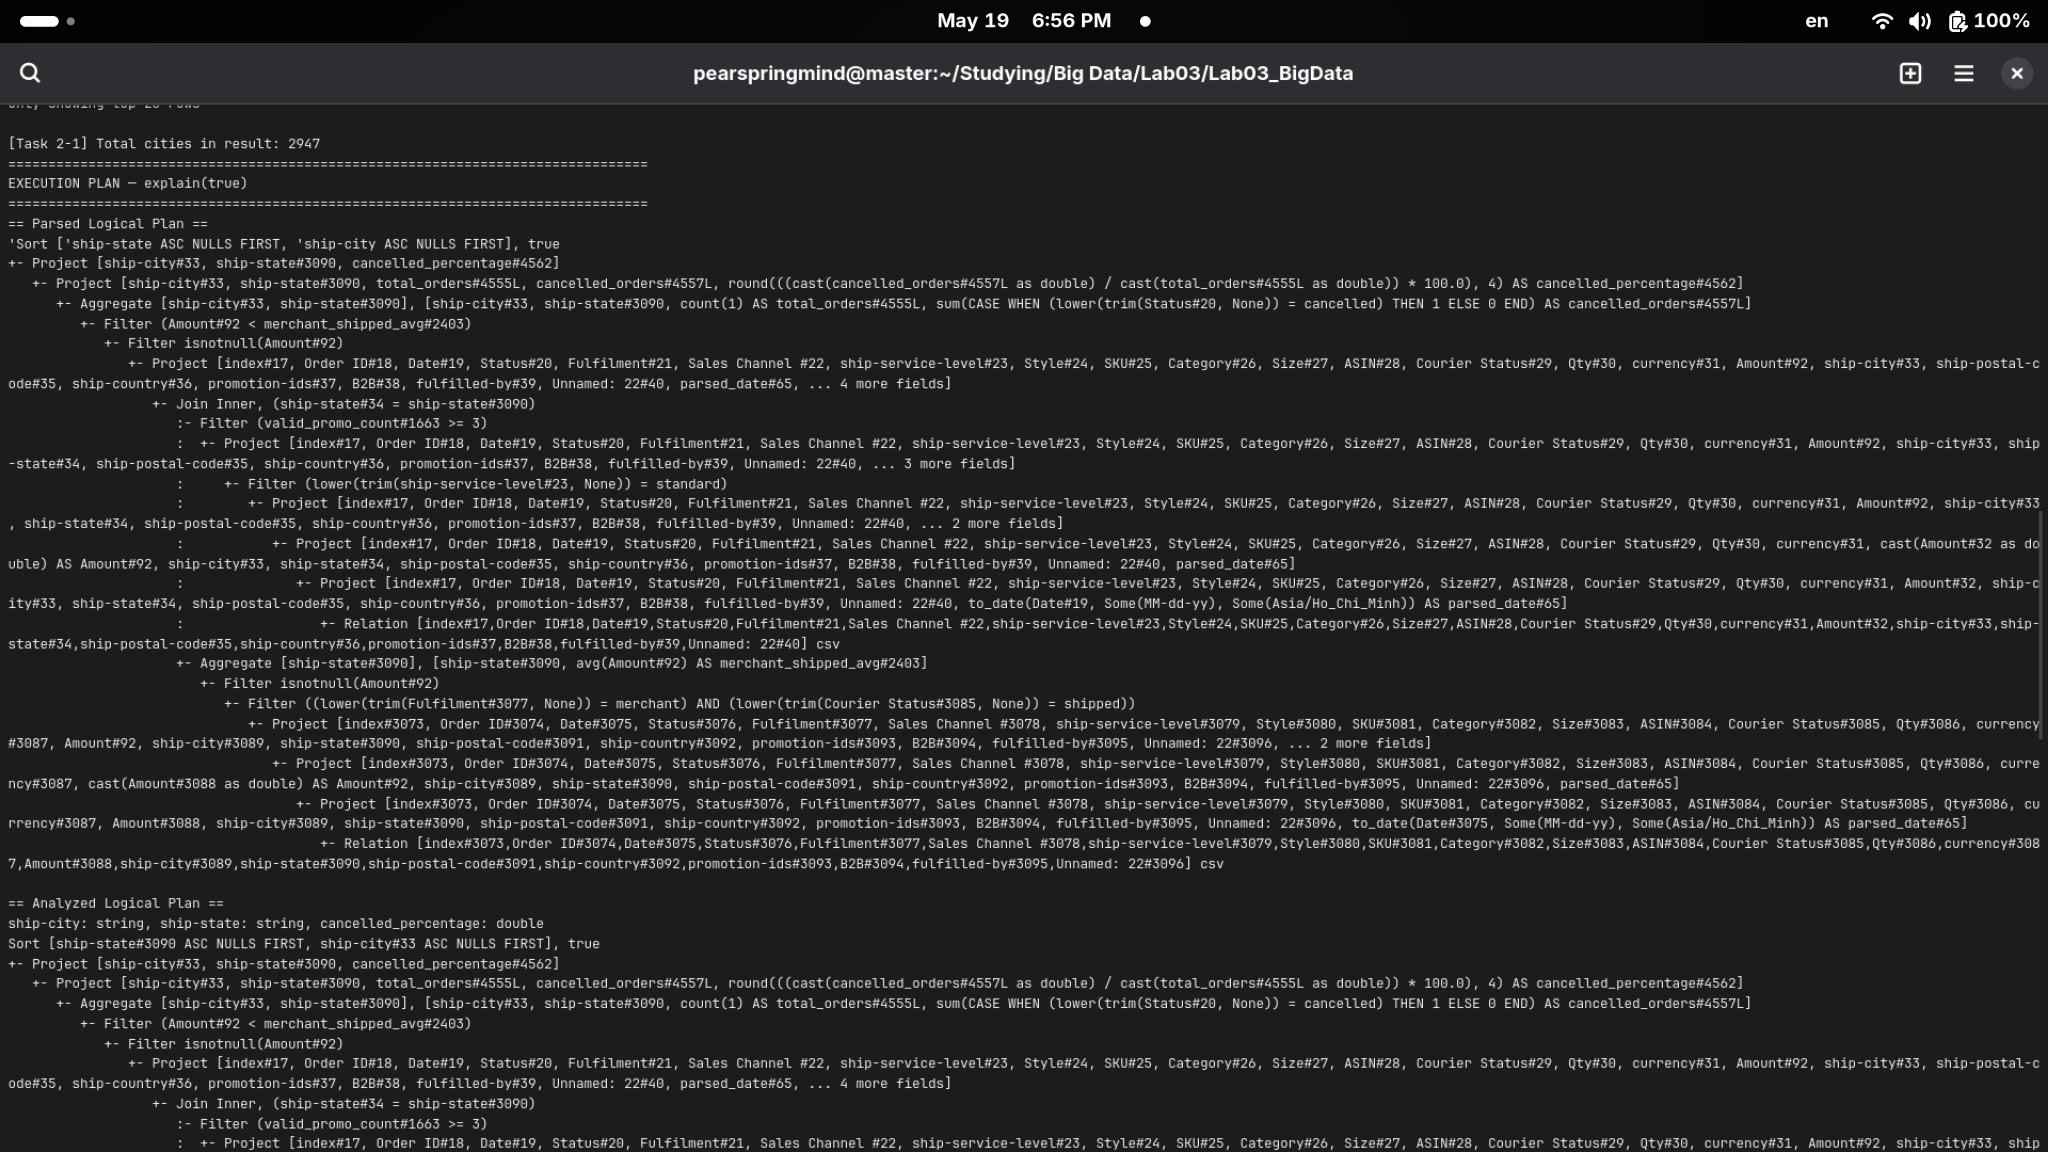
\includegraphics[width=0.9\textwidth]{img/2-1/explain_plan.png}
    \caption{Kế hoạch thực thi vật lý (Execution plan) của Task 2.1}
    \label{fig:task2_1_explain_plan}
\end{figure}

\begin{figure}[H]
    \centering
    
\includegraphics[width=0.9\textwidth]{img/2-1/output_preview.png}
    \caption{Một phần nội dung tệp Parquet kết quả đầu ra \texttt{Task\_2-1.parquet}}
    \label{fig:task2_1_output_preview}
\end{figure}
